\documentclass{standalone}
\usepackage{tikz}
\begin{document}
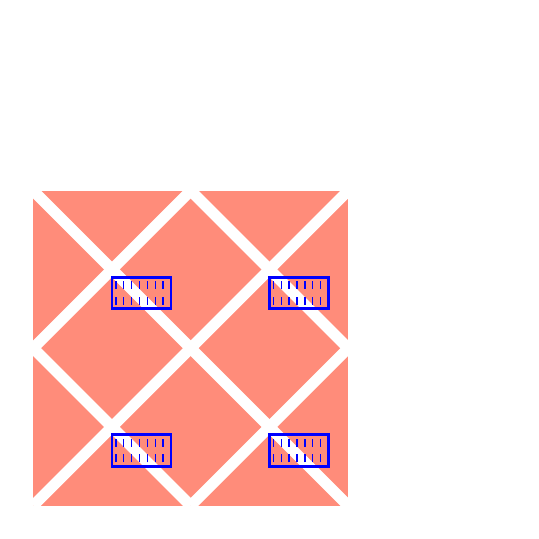
\begin{tikzpicture}[scale=0.5]
    % Define colors
    \definecolor{lightred}{RGB}{255, 213, 170}
    \definecolor{darkred}{RGB}{255, 140, 122}
    \definecolor{blue}{RGB}{0, 0, 255}

    % Draw shaded red areas
    \fill[lightred] (0,0) rectangle (8,8);
    \fill[darkred] (0,0) rectangle (4,4);
    \fill[darkred] (4,4) rectangle (8,8);
    \fill[darkred] (0,4) rectangle (4,8);
    \fill[darkred] (4,0) rectangle (8,4);
    
    % Draw diagonal lines to create the checkerboard pattern
    \foreach \i in {0,4,8} {
        \foreach \j in {0,4,8} {
            \draw[white, line width=4] (\i, \j) -- (\i+4, \j+4);
            \draw[white, line width=4] (\i+4, \j) -- (\i, \j+4);
        }
    }
    
    % Draw blue rectangles and patterns
    \foreach \x/\y in {2/5, 6/5, 2/1, 6/1} {
        % Blue rectangles
        \draw[blue, line width=1] (\x,\y) rectangle (\x+1.5,\y+0.8);
        % Blue patterns inside the rectangles
        \foreach \i in {0.1,0.3,...,1.4} {
            \draw[blue, line width=0.5] (\x+\i,\y+0.1) -- (\x+\i,\y+0.3);
            \draw[blue, line width=0.5] (\x+\i,\y+0.5) -- (\x+\i,\y+0.7);
        }
    }
\end{tikzpicture}
\end{document}